%---------------------------------------------------------------
%---------------------------------------------------------------
\chapter{Erzeugung der Dinge, die nicht von PCA vorgegeben sind}

Ein Punkt im PCA-Raum gibt schon viele Eigenschaften des zu generierenden Skeletts vor. Zu den Dingen, die noch festgelegt werden müssen, zählen \zb die Anzahl und Anordnung der Wirbel und Rippen und vor allem die Ausrichtung der Extremitäten.

%-----------------------------------------------
\section{Ausrichtung der Extremitäten}
\label{section:extremity_generation}

% Allgemeine Schwierigkeit Extremitäten zu positionieren
Das Skelett soll in einer Art Ruheposition dargestellt werden. Im Allgemeinen ist aber nicht klar wie die Ruheposition einer Extremität aussieht. Das ist schon allein daran zu erkennen, dass auf Darstellungen von Wirbeltierskeletten Flügel manchmal ausgestreckt und manchmal eingefaltet sind. Auch Beine sind meist so angeordnet, dass es aussieht als würde das entprechende Tier gerade laufen. Dies ist auf Abbildung \ref{klippschliefer} am Beispiel des Klippschliefers sehr gut zu sehen.

 \begin{figure}
  \centering
  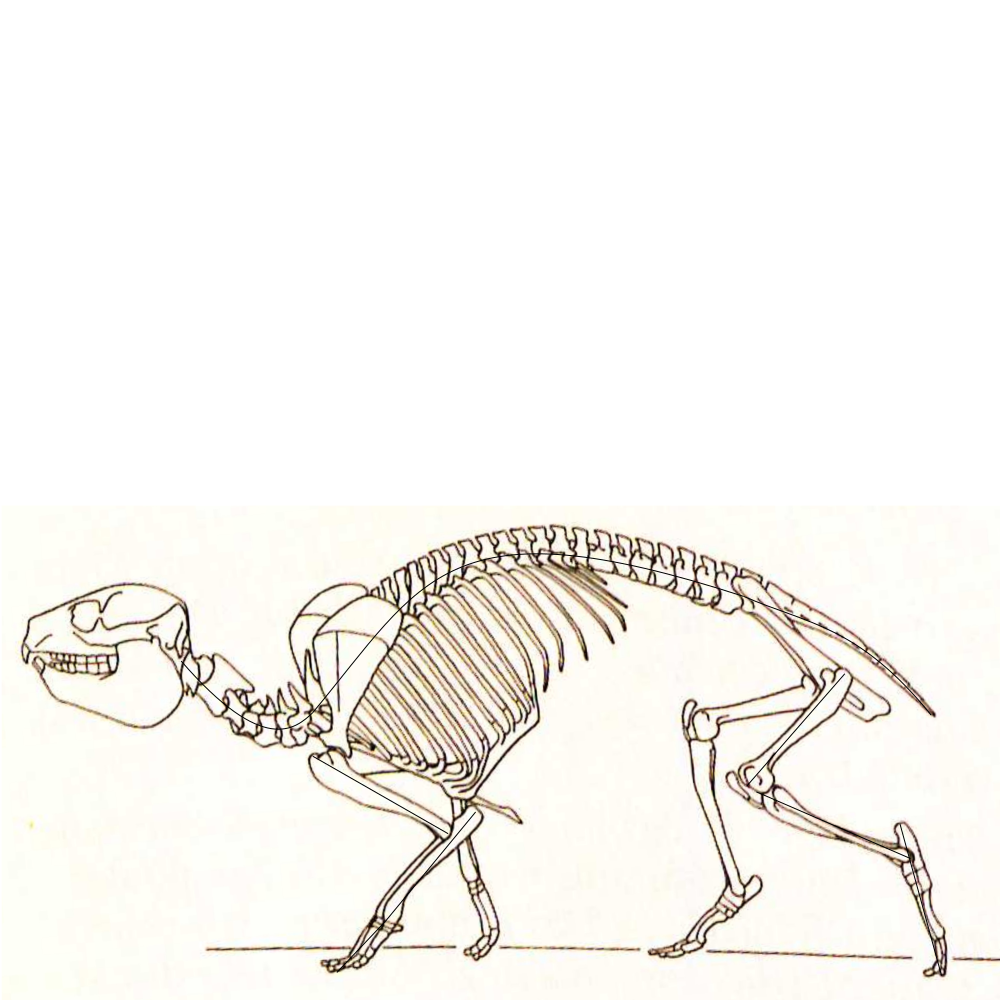
\includegraphics{../PCA/Skelettbilder/Klippschliefer.jpg}
  \caption{Skelett eines Klippschliefers. Dieses Bild wurde auch als Eingabe für die PCA verwendet.}
  \label{klippschliefer}
 \end{figure}

Wie in Kapitel \ref{chapter:pca} zur PCA schon erwähnt, ist es deshalb auch schwer möglich die Ausrichtung der Extremitäten \bzw die Winkel an den Gelenken als zusätzliche Dimension in den PCA-Raum mitaufzunehmen.

Die Positionierung der Extremitäten bleibt also ein Problem mit unklaren Anforderungen und vielen Freitheitsgraden.

% Einteilung in Kategorien
Ein erster Schritt an das Problem heranzugehen, ist es in kleinere Unterprobleme zu zerteilen:
Extremitäten können anhand ihrer Funktion in vier Kategorien eingeteilt werden:
Flügel, Flossen, Extremitäten mit Bodenkontakt (im Folgenden als Beine bezeichnet), und Extremitäten ohne Bodenkontakt (im Folgenden als Arme bezeichnet).

Für Flügel, Flossen und Arme gibt es keine besonderen Anforderungen außer, dass sie als solche zu erkennen sein sollten. Deshalb werden sie nach folgenden simplen Anweisungen orientiert:
\todo{Beispielbilder?}
\begin{itemize}
 \item Flossen: Ausrichtung gerade nach hinten (orientiert an Welt-x-Achse)
 \item Arme: Der Oberarm zeigt senkrecht nach unten (orientiert an Welt-y-Achse), im Ellenbogengelenk ist ein $90^{\circ}$ Winkel und die Hand verlängert Unterarm nach vorne.
 \item Flügel: Jedes beteiligte Gelenk hat ein Intervall mit festen Grenzen, aus dem zufällig ein Winkel gewählt wird.
\end{itemize}

Nun bleibt nur doch die Ausrichtung der Beine, für die die zusätzliche Anforderung gilt, dass sie den Boden berühren sollen.


%- - - - - - - - - - - - - - - - - - 
\subsection{Berechnung der Bodenhöhe}

% Warum nicht Höhe 0?
Zunächst könnte man davon ausgehen, dass der Boden einfach auf Höhe null sein sollte. Das Problem hierbei ist aber, dass die von der PCA berechneten Längen für die Extremitäten meist so kurz sind, dass die Beine dann den Boden nicht mehr erreichen würden. Das liegt daran, dass auf den Bildern, die als Eingabebeispiele für die PCA verwendet wurden, der Boden meistens auch nicht ganz am unteren Rand ist. Hier würde rigoroses Abschneiden der Bilder auf Fußhöhe wahrscheinlich helfen, es würde aber in vielen Fällen auch ein Großteil der Füße fehlen.

% Berechnung
Die Höhe des Bodens wird also anhand der von der PCA generierten Längen der Extremitäten festgelegt.
Theoretisch würde es reichen einfach das kürzeste Bein im komplett ausgestreckten Zustand zu betrachten und den Boden auf die Höhe dessen Endpunkts festzulegen.
Das führt aber zu unnatürlich aussehenden Beinen, da das kürzeste Bein einfach gerade nach unten führt.

Deshalb wird nur ein bestimmter Anteil der Länge der Beine betrachtet. So wird erzwungen, dass die Beine, wenn sie auf dem neu definierten Boden stehen, auch etwas gekrümmt sind.

\todo{Wkt für Verse auf Boden erklären}


%- - - - - - - - - - - - - - - - - - - - - - - - -
\subsection{Algorithmus zur Ausrichtung der Beine}

\todo{Absatz über IK, lcp (linear complementary problem) (nicht Hauptaugenmerk / Ziel der Arbeit ist etwas anderes / reicht für Proof of Concept, bei Animationen muss große Maschinerie sowieso nochmal angeworfen werden)}

% iterativ, Drehrichtung
Der hier verwendete Algorithmus zur Ausrichtung der Beine geht iterativ vor.
In jedem Schritt wird für jedes Gelenk berechnet ob sein Winkel vergrößert oder verkleinert werden muss um den dazugehörigen Knochen näher zum Boden zu bewegen.
Mit dem "`dazugehörigen"' Knochen ist hier derjenige der beiden an das Gelenk anschließenden Knochen gemeint, der das Kindelement des anderen ist.
Die Drehrichtung lässt sich relativ leicht herausfinden indem die Ausrichtung des Knochens mit der Welt-y-Achse verglichen wird. Je senkrechter der Knochen ausgerichtet ist, desto ausgestreckter ist das Bein.
\todo{Schaubilder für verschiedene Gelenkarten?}

% Einschränkungen der Gelenke
Zusätzlich gibt es für jedes Gelenk und jeden Freitheitsgrad einen minimalen und einen maximalen Winkel, der eingenommen werden kann. Dieses Intervall hängt von den anatomischen Möglichkeiten des Gelenks ab und von den Winkeln, die in einer "`sinnvollen"' Ruheposition eingenommen werden können. 
\todo{ist das überhaupt eine Einschränkung?}
\todo{Problematik mit lokalen Winkelkonstraints vs. globalen Berechnungen für Abstand zum Boden}

% Startposition, Bewegungseinschränkungen
Die Startposition der Extremität ist maximal angewinkelt. Die Gelenke beginnen also mit ihren kleinst- \bzw größtmöglichen Winkeln. In den folgenden Iterationen wird dann derjenige Endpunkt der Extremität dem Boden genähert, der zum Schluss Bodenkontakt haben soll.
Ohne weitere Einschränkungen kann es nun passieren, dass unnatürliche Positionen auftreten, in denen \zb der Fußspann näher am Boden ist als die Fußsohle.
Oder es kann passieren, dass ein Knochen, der über die positive Welt-y-Achse hinaus gedreht wird. Das Problem dabei ist, dass die Einschränkungen an den Gelenken nicht zulassen, dass der Knochen sich unbegrenzt in diese Richtung weiterdreht und der Knochen dann "`feststeckt"'. Deshalb wird nach jeder Drehung festgestellt ob so eine Situation eingetreten ist und wenn ja, wird die Drehung rückgängig gemacht.
Die Drehung wird ebenfalls rückgängig gemacht, falls sie bewirkt, dass die Knochen unterhalb der Bodenhöhe landen.
\todo{Beispielbilder}
So ist zu jeder Zeit garantiert, dass die Knochen auf der "`richtigen"' Seite der y-Achse liegen und nicht unterhalb der Bodenhöhe sind. % Invarianten

% Verkleinerung der Größe der Drehwinkel
In jeder Iteration werden die Winkel, um den die Gelenke gedreht werden, um einen bestimmten Anteil verkleinert. Zu Beginn soll, mit den großen Veränderungen, eine grobe Ausrichtung der Gelenke vorgenommen werden, die dann immer weiter verfeinert wird.
In der ersten Iteration startet der Algorithmus mit $40^{\circ}$. Später sind es dann jeweils $\frac{6}{7}$ davon.
Diese Zahlen sind durch Ausprobieren zu Stand gekommen. Der Startwinkel darf nicht zu klein sein, weil die Gelenke sonst ihre Zielpositionen nicht erreichen können. Ist der Startwinkel zu groß, bewirkt es in vielen Fällen nur, dass die Drehung nicht durchgeführt werden kann, weil die oben genannten Randbedingungen verletzt werden.
Die Verkleinerung des Winkels darf nicht zu schnell geschehen, weil dann wiederum nicht die Endposition nicht erreicht werden kann. Wenn sie zu langsam geschieht passiert in vielen Schritten wiederum nichts wegen verletzter Randbingungen.

Falls sich der Abstand zum Boden also kaum verändert, liegt die Vermutung nahe, dass die Gradzahl zu groß ist und deshalb alle möglichen Winkeländerungen invalide sind. Deshalb wird in diesem Fall die Gradzahl für die nächste Iteration stärker verkleinert (halbiert).

\todo{Wkten für Gelenke, Vorteil?}

% Zweiter Freiheitsgrad
Theoretisch haben das Hüft- und das Schultergelenk nicht nur einen, sonder zwei Freiheitsgrade. Das lässt sich auch als zweite Art von Gelenk im Code abbilden. Allerdings liefert der Algorithmus dann oft seltsam anmutende breitbeinige Tiere.
Deshalb wurde der zweite Freiheitsgrad hier außen vor gelassen.
Obwohl es natürlich in der Natur auch viele Tiere mit nach außen gestellten Beinen gibt, wie \zb Echsen.
% + max angewinkelte Pos komisch und Drehrichtung ändert sich je nach anderen Winkel


% \begin{algorithm}
%  \caption{Beinalgorithmus}
%  \label{beinalgo}
%  
%  \begin{algorithmic}
%     \STATE{step = 0\\
%     maxSteps = 50\\
%     angleStepSize = $40^\circ$}
% 
%     \WHILE{floor not reached and step < maxSteps}
%         \FORALL{joints}
%             \IF{child bone of joint has not reached floor and movement nearer to floor possible}
%                 \STATE try change joint angle
%             \ENDIF
%         \ENDFOR
%         \IF{angleStepSize > eps}
%             \STATE reduce angleStepSize
%         \ENDIF
%     \ENDWHILE
%  \end{algorithmic}
% \end{algorithm}
\todo{Pseudocode?}

\todo{Evaluierung}
\begin{itemize}
 \item generierte Extremitäten mit echten Positionen vergleichen, diskutieren\\
    schlimmes Beispiel für Beinalgo: Brachiosaurus (+ Elefant?)
 \item keine wissenschaftliche Argumentation für Änderungen am Beinalgo, nicht klar was Verbesserungen wären; Beine müssen für Animation, Muskelgeneration etc sowieso nochmal angefasst werden -> future work
 \item Bei Skeletten, die sehr kurze Beine haben, funktioniert der Algorithmus teilweise nicht besonders gut:
  \begin{itemize}
   \item Beinstartposition kann schon unter Bodenhöhe sein, wenn Beine sehr unterschiedlich lang / Startpunkte sehr unterschiedlich hoch sind (Berechnung der Bodenhöhe erklären). Beispiel dafür: Dimetrodon
   \item Bei Berechnung der Bodenhöhe wird von Kontrollpunkten der Bezierkurve aus gemessen (da Position der Hüfte/Schulter noch nicht klar). Deshalb kann es bei sehr kurzen Beinen sein, dass Abstand zwischen Boden und Gelenk zu groß ist und Boden so nicht erreichbar ist.
   \item Bei sehr kurzen Knochen ändert sich der Abstand zum Boden durch Drehung der Gelenke nicht so stark wie bei langen Knochen, deshalb wird Winkel öfter halbiert, was in diesem Fall aber kontraproduktiv ist. Aus diesem Grund schafft der Algorithmus es dann nicht mehr die Knochen in die richtige Lage zu bringen. (der Bewegungsspielraum wird zu stark eingeschänkt)
   \item bei ganz kurzen Beinen (Gesamtlänge unter 5) macht es keinen Sinn sie anzuordnen (außerdem gibt es den gleichen Effekt wie oben schon erwähnt)
   \item Bei kurzen Arm/Beinknochen kann es dazu kommen, dass der Oberarm nicht näher zum Boden kann, aber Unterarm (+Hand) durch das Gelenkoffset über dem Boden schweben und nicht näher heran kommen (siehe Krokodil screenshot)
  \end{itemize}
\end{itemize}

%--------------------------------------
\section{Zusätzliche Ansatzpunkte für Extremitäten}

Ansatzpunkte für Extremitäten sind natürlich zunächst der Hüftgürtel und der Schultergürtel. Um auch die Generierung fantastischer Tiere zu ermöglichen, ist es aber Möglich dies zu erweitern.\\
\todo{andere Möglichkeiten fantastische Tiere zu generieren?}

Eine einfache Möglichkeit ist hier zunächst die Anzahl der möglichen Extremitätenpaare von zwei auf vier zu erhöhen, indem einfach an der Hüfte und der Schulter jeweils zwei Paare ansetzen dürfen. Dafür wurden einfach an der Hüfte \bzw der Schulter mehrere Gelenke mit ein wenig Abstand angelegt, an denen Extremitäten ansetzen können.
Flügel und Arme dürfen hierbei weiterhin nur an der Schulter ansetzen, Beine und Flossen an beiden Stellen. Der Grund dafür ist, dass die meisten generierten Skelette seltsam wirken, wenn an der Hüfte Flügel oder Arme ansetzen und dafür an der Schulter Beine beginnen. Das liegt daran, dass existierende Tiere mit Flügeln oder Armen ihren Schwerpunkt im hinteren Bereich haben und sie auf den Hinterbeinen stehen.

% mehr Extremitätengürtel auf dem Rücken
Eine Überlegung war auch zwischen Schulter und Hüfte weitere Extremitätengürtel anzubringen. Das stellt sich aber als schwierig heraus. Die Wirbelsäule ist zwischen Hüfte und Schulter nach oben geschwungen und im Bauchraum befinden sich die meisten Organe des Tieres. Ein zusätzlicher Extremitätengürtel würde den Bauchraum einschränken. Außerdem wirkt dann auch die nach oben geschwungene Wirbelsäule anatomisch seltsam.
"`Verdoppelt"' man die Schwingung der Wirbelsäule und hängt einfach einen weiteren Rücken hinten oder vorne an, so wirkt es ebenso seltsam, da dann die "`Höcker"' der Wirbelsäule für das Tier wahrscheinlich nicht wirklich ein Vorteil sind und nur die Fortbewegung erschweren.

% zweiter Schultergürtel
Eine weitere Idee, die auch umgesetzt wurde, ist, eine Art Zentauren zu ermöglichen. Hat das Tier einen Hals, der lang genug ist, kann darauf ein weiterer Schultergürtel kurz unterhalb vom Kopf angebracht werden. An diesem Schultergürtel dürfen dann keine alle Arten von Extremitäten außer Beinen ansetzen. Das wirkt tatsächlich meist auch anatomisch einigermaßen sinnvoll.

%- - - - - - - - - - - - - - - - - - - 
\subsection{Anordnung der Extremitäten}

\begin{itemize}
 \item Anzahl der Extremitäten orientiert sich an Benutzereingabe
 \item falls keine Benutzereingabe, dann orientiert es sich an den von der PCA ausgespuckten Wahrscheinlichkeiten für Beine und Flügel
 \item die Position jeder Extremität wird zufällig aus der Menge der möglichen Positionen ausgewählt. Ist für eine Extremität kein Platz mehr, wird geschaut, ob andere Extremität an eine andere Position wechseln kann um Platz zu schaffen
 \item da Positionen nicht deterministisch kommt es bei Tieren mit mehreren möglichen Anordnungen zu unterschiedlichen Ergebnissen bei gleicher Eingabe
 \item da die Anzahl der Arme und Flossen nicht mit PCA erhoben kann sie für die Eingabebeispiele der PCA nicht rekonstruiert werden. Deshalb kann Benutzer hier eigene Angaben machen.
 \item nachdem Extremitäten zugeteilt wurden, werden sie nochmal "`verteilt"', damit nicht \zb zwei Beine an Hüfte aber keins an Schulter \todo{sinnvoll?}
 \item wenn es keine Angabe für die Anzahl der Flügel gibt, werden diese mit der PCA Wkt generiert, aber max ein Paar pro Schultergürtel; bei Beinen wir die Wkt (kann auch 2 sein) auf- oder abgerundet
 \item Arme werden ebenfalls mit Flügelwkt generiert (auch max 1 pro Schultergürtel)
 \item Flossen werden in komplett leere Extremitätengürtel generiert, wenn sie nicht zu lang wären
\end{itemize}


%---------------------------------------------------
\section{Weitere Dinge, die generiert werden müssen}

\begin{itemize}
 \item Wirbel
 \item Rippen (wieviele Rippen, wie lang ist Brustkorb in x-Richtung)
 \item Kopf
 \item Schulter 
\end{itemize}
